
\chapter{Contribution} % Main chapter title

\label{Chapter6} % Change X to a consecutive number; for referencing this chapter elsewhere, use \ref{ChapterX}

%----------------------------------------------------------------------------------------
%	SECTION 1
%----------------------------------------------------------------------------------------

\section{Unity}

Unity le logiciel que j'utilise pour développer mon framework, c’est est un moteur de jeu multiplateforme (smartphone, ordinateur, consoles de jeux vidéo et Web) développé par Unity Technologies. Il est l'un des plus répandus dans l'industrie du jeu vidéo, aussi bien pour les grands studios que pour les indépendants du fait de sa rapidité aux prototypages et qu'il permet de sortir des jeux sur tous les supports.


~\par
En terme d’intelligence artificielle, ce dernier propose une multitude de fonctionnalités notamment basées sur l’apprentissage (Machine Learning) afin de construire des agents autonomes, conscients de leur environnement et qui interagissent avec selon des paramètres précis, objectifs, actions et réactions.

~\par
L’un des facteurs qui m’ont poussé à l’utiliser et aussi le fait qu'il a la particularité de proposer une licence gratuite dite « Personal » avec quelques limitations de technologie avancée au niveau de l'éditeur, mais sans limitation au niveau du moteur.  



\section{Le Jeu open source “Do not shoot Aliens” - Jeu Mobile}

L'idée principale derrière est de complètement transformer les mécanismes que l’on attend d'un jeu de tir classique, en effet,  au lieu de viser et de tirer afin de vaincre ses ennemis, le personnage du joueur est un peu agressif et décide de tirer sur tout ce qui est autour de lui. 

Le but du joueur est d’atteindre le moins de personnages extraterrestres pour ne pas les contrarier.

Plus les extraterrestres sont touchés, plus le jeu sera difficile, car le joueur devra les frapper une seconde fois pour les arrêter. [Figure \ref{fig:7.2}] 

La victoire est basée sur le fait d’accumuler le plus de points possible en allant de checkpoint en checkpoint.

\begin{figure}[th]
\centering
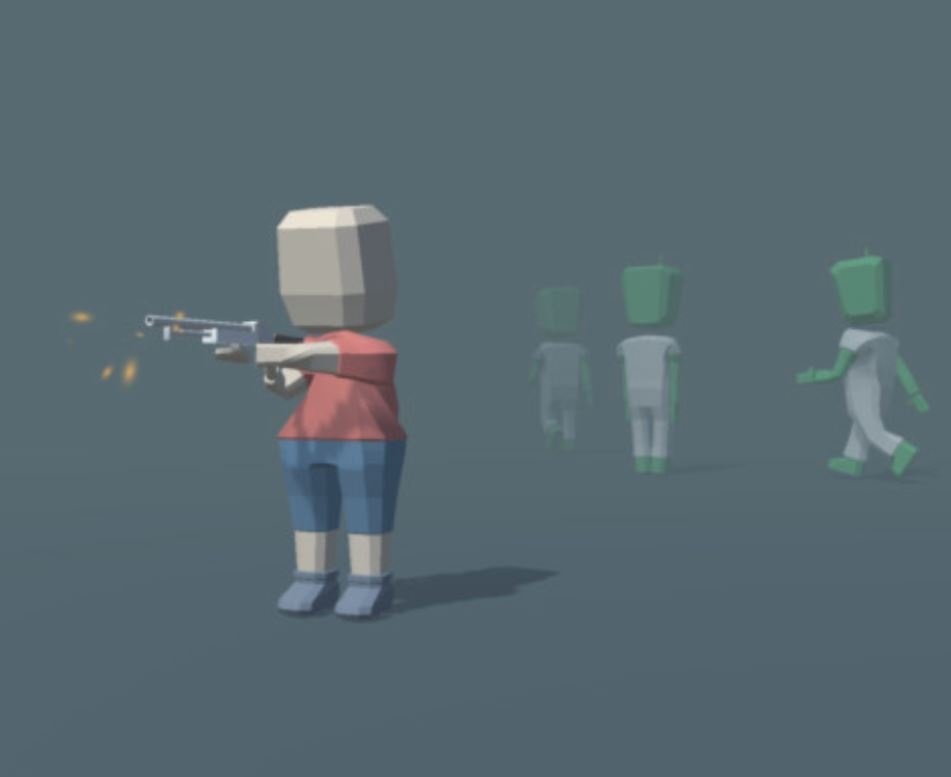
\includegraphics{Figures/72unity.JPG}
\decoRule
\caption[Icon du jeu "Do Not Shoot Aliens"]{Icon du jeu "Do Not Shoot Aliens"}
\label{fig:7.2}
\end{figure}

\section{Langage de programmation}

Chaque agent de ce jeu, que ce soit le personnage principal contrôlé par le joueur ou les agents autonomes représentés ici par les ennemis et même l’environnement ou les objets qui interagissent avec les agents, est géré par un code source qui lui est propre, ce dernier est écrit en C-Sharp, un langage de script qui permet ensuite au moteur de jeu de le compiler et de l'interpréter, et cela, afin de garantir les meilleures performances de jeu.

~\par
Ce langage est orienté objet, ce qui fait sens car tous les objets, environnements, agents ou encore joueurs sont effectivement des objets 3D, ayant des paramètres qui leur sont propres ( Vitesse, durée de vie, couleur, objectif ) ainsi que de nombreuses fonctions ( marcher, courir, frapper, sauter etc…) qui leur permettent d’effectuer des actions, cette définition nous renvoie au concept de classe, variables de classes et méthodes de classe présentes dans les langages orientés objet.


\section{Description des agents autonomes présents dans le jeu}

Le scénario typique pour la formation d’agents dans des environnements virtuels consiste à avoir un environnement et un agent uniques qui sont étroitement couplés. Les actions de l'agent modifient l'état de l'environnement et lui procurent des récompenses. \parencite{unity2}  

~\par
Dans notre cas, les agents ont pour environnement l’esplanade sur laquelle ils circulent, ils peuvent effectuer des actions par exemple:  marcher doucement, courir ou encore attaquer.
 
 
~\par 
Leur objectif initial est celui de rester “tranquille”, en effet, tant qu’ils ne sont pas touchés, ils conservent leur démarche lente et continuent de circuler de manière hasardeuse (fonction random qui génère leur position dans l’espace).

~\par
Par contre s'ils venaient à être touchés par les balles du joueur principal, leur comportement change et leur objectif aussi, ils se concentrent alors principalement sur l’attaque du personnage principal afin de s’en débarrasser.

On peut identifier ici un exemple de BDI (décrit plus haut): 

\begin{itemize}
\item Leur "Belief" ( ou croyance ) initiale est de croire que leur environnement est inoffensif, c’est leur vision du monde.
\item Ce qui engendre leur désire ou encore leur objectif, qui est de circuler dans l’environnement qui les entoure, ceux-ci décrivent l'état du monde parfait dans lequel ils aimeraient évoluer.
\item Leur "Intention" est ici le plan d’action en cours d'exécution, c’est-à-dire, le fait de déambuler sur l’esplanade.
\end{itemize}


~\par
Comme vu précédemment, tout changement dans leur environnement peut produire un changement dans leur perception de ce dernier, et donc engendrer un nouveau plan d’action, c’est sur ce principe que je me base afin d’appliquer à ces gens différents paramètres qui leur permettront de réagir à leur nouvel environnement. 

\section{Application de paramètres de prises de décisions en milieu naturel (NDM) aux agents BDI}

Afin d’appliquer ces paramètres, je procède de la manière suivante [Figure \ref{fig:75}] : 

\begin{itemize}
\item Je déclare des paramètres qui permettent d’évaluer l’état émotionnel des agents lors des différents changements de l’environnement.
\item Ces variables sont: la peur, la joie, la tristesse et la colère qui sont des booléens.
\item Chaqu’une de ces variable a, à son tour des paramètre qui lui sont étroitement liées: la vitesse de la démarche, ainsi que la couleur des agents.
\item En l'occurrence, la couleur associée à la joie est le jaune.
\item Celle associée à la tristesse est le bleue.
\item Celle associée à la colère est le rouge.
\item Celle associée à la peur est le vert. [Figure \ref{fig:751u}, Page \pageref{fig:751u}]
\end{itemize} 

\begin{figure}[th]
\centering
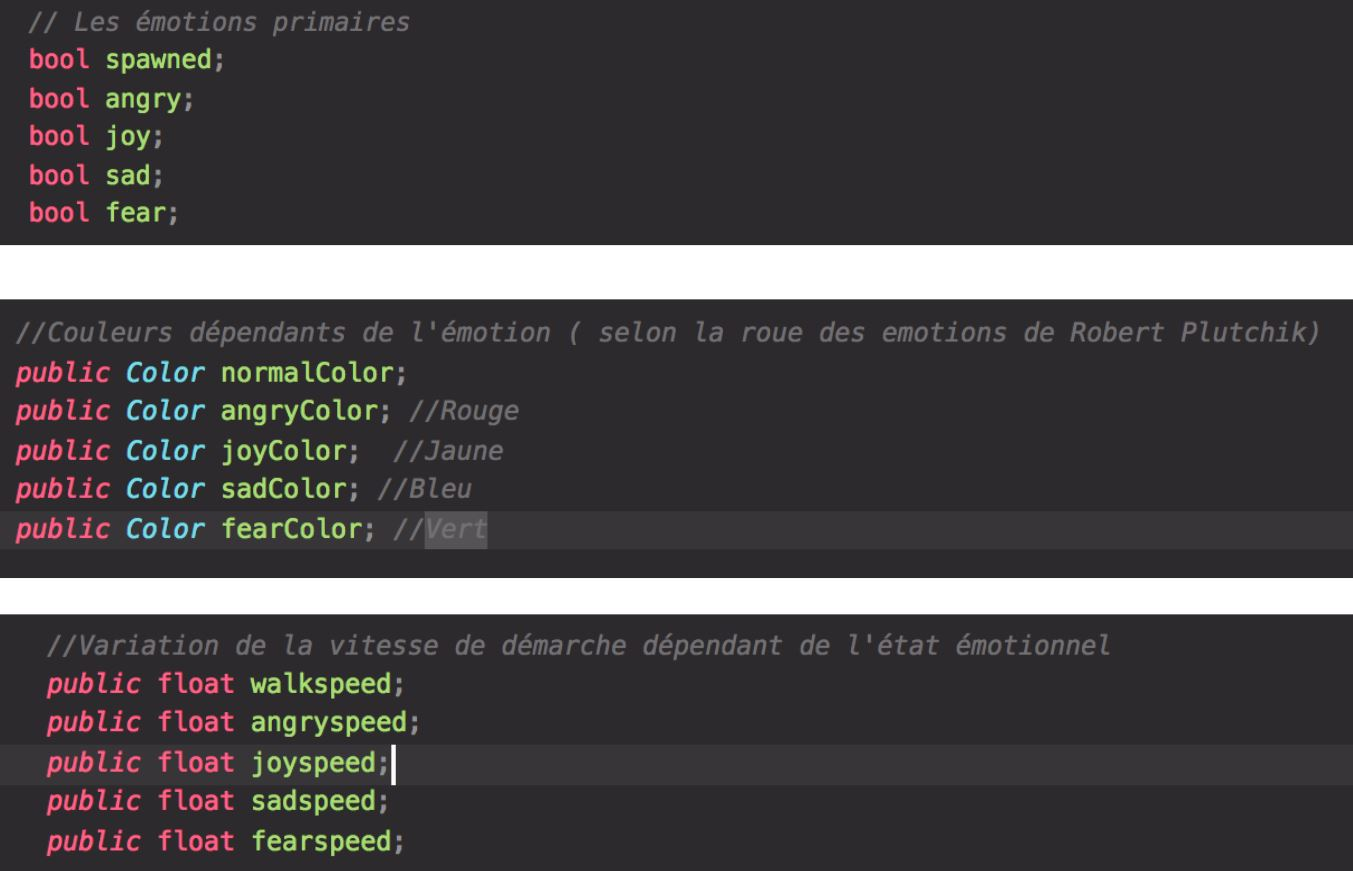
\includegraphics{Figures/75unity.JPG}
\decoRule
\caption[Déclaration des variables]{Déclaration des variables}
\label{fig:75}
\end{figure}



\begin{figure}[th]
\centering
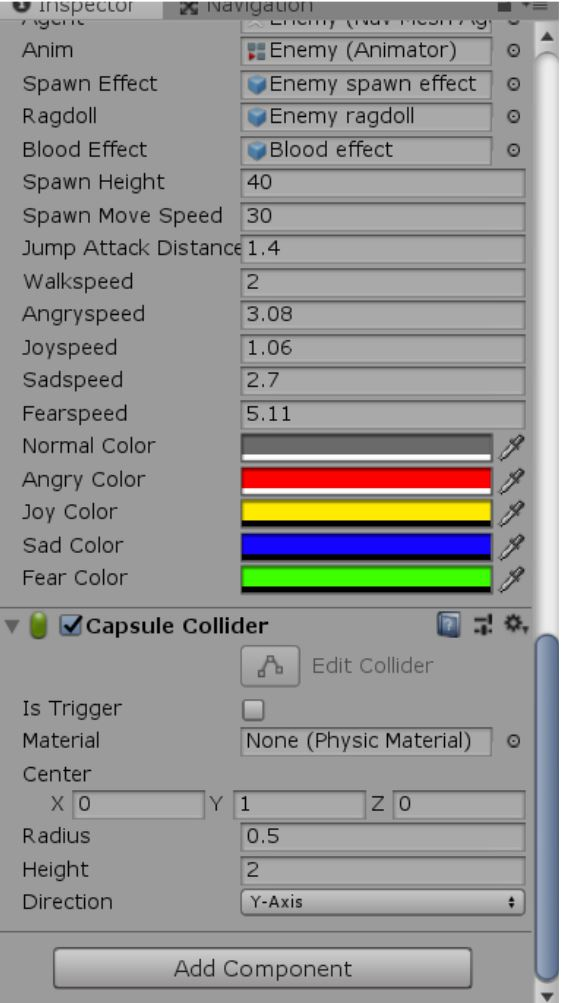
\includegraphics{Figures/751unity.JPG}
\decoRule
\caption[Fenêtre Unity, Valeurs des paramètres]{Fenêtre Unity, Valeurs des paramètres}
\label{fig:751u}
\end{figure}


\subsection{Première expérimentation}

Lors de ma première expérimentation, j’ai décidé d’établir une distance critique entre le joueur et les agents autonomes, lorsque ce dernier est très proche d’eux, qui serait synonyme de tristesse pour ces derniers, sentiment lié au fait de savoir que le jour peut à tout moment les toucher.


\begin{figure}[th]
\centering
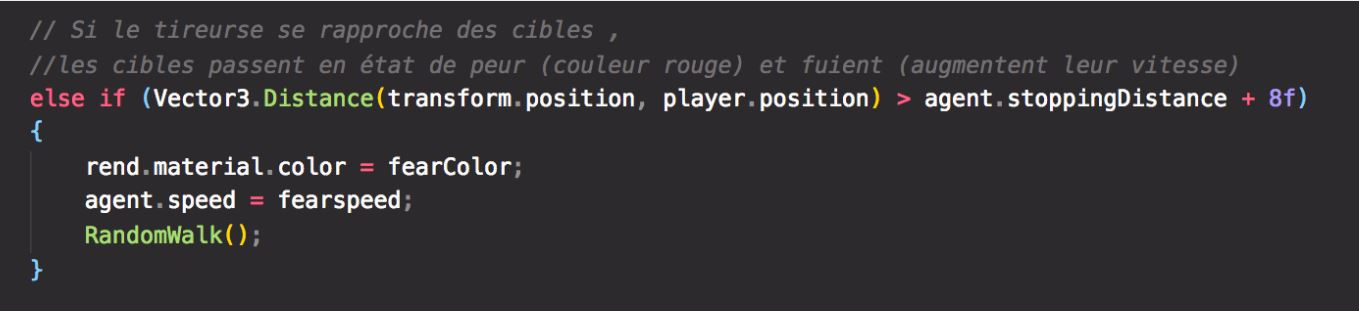
\includegraphics{Figures/fonctdist.JPG}
\decoRule
\caption[Code source implémentant une courte distance ]{Code source implémentant une courte distance entre le jouer et l'agent}
\label{fig:751}
\end{figure}



~\par
La distance est exprimée ici par la position de l’agent en mode “stop” ou à l'arrêt (qui survient lorsque l’agent rencontre sur son chemin ou “path” le joueur) et le joueur lui-même, à laquelle on ajoute un delta en nombre flottant représenté ici par le 8f, il suffit ensuite de varier ce nombre flottant afin d’augmenter ou de diminuer le delta, et de calculer la distance qui sépare les agents autonomes(plus ou moins loin selon le delta) du joueur. 

~\par
Le résultat souhaité est de pouvoir appliquer un changement de couleur aux agents suivant l’émotion qu’ils ressentent, dans la figure \ref{fig:751}, c’est la peur, la couleur de l’agent prend donc la couleur associée à la peur [Figure \ref{fig:bichi1}] une fois que ce dernier est à une distance équivalente à un delta de 8, ce dernier change aussi de vitesse de démarche et adopte un rythme plus élevé lui permettant d'échapper au joueur au fur et à mesure que celui-ci se rapproche. ( La vitesse liée à la peur est plus élevée que celle liée à la démarche dite "normale" comme le montre la figure \ref{fig:751u} ).


\begin{figure}[th]
\centering
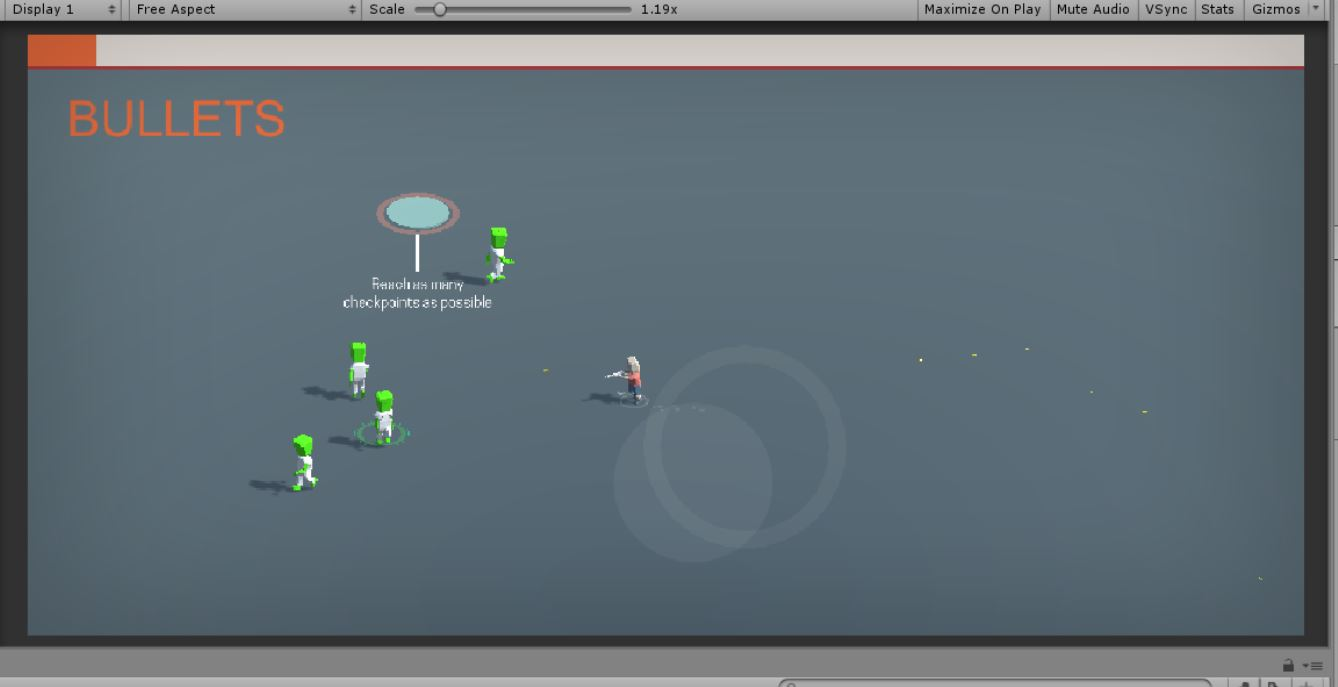
\includegraphics{Figures/bichi1.JPG}
\decoRule
\caption[Visualisation d'agents en état de peur]{Visualisation d'agents en état de peur}
\label{fig:bichi1}
\end{figure}



\subsection{Deuxième expérimentation}

On ajoute cette fois-ci à l'expérience précédente un nouveau facteur émotionnel, celui de la joie.
Suivant le même principe que précédemment, on définit un delta qui permet de calculer la distance entre le joueur et l’agent autonome, celui-ci est de 20f, une distance assez élevée. [Figure \ref{fig:fonct2}]

\begin{figure}[th]
\centering
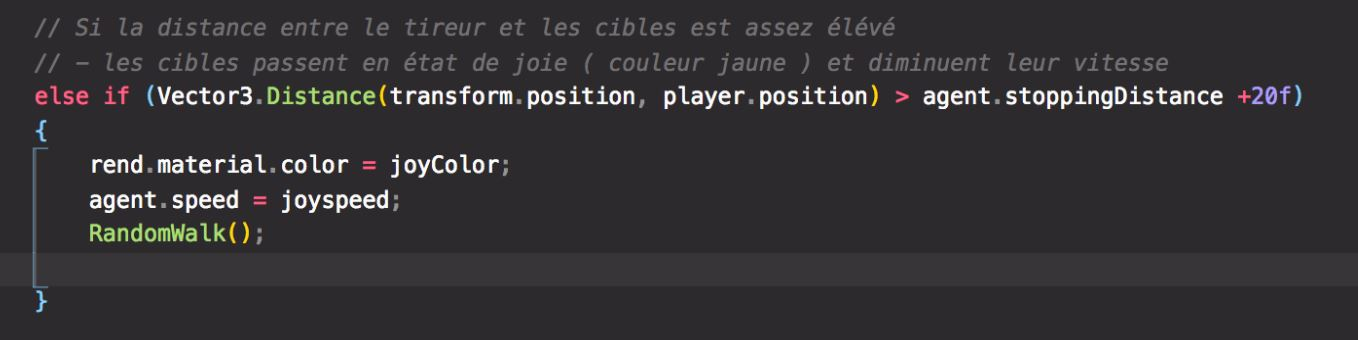
\includegraphics{Figures/fonct2.JPG}
\decoRule
\caption[Code source implémentant une longue distance]{Code source implémentant une longue distance entre le jouer et l'agent}
\label{fig:fonct2}
\end{figure}



~\par
Le résultat souhaité est de pouvoir appliquer un changement de couleur aux agents à l’instant où cette distance entre eux et le joueur est atteints.

~\par
La couleur de ces derniers devient alors jaune, et leur vitesse passe à un rythme beaucoup moins élevée. [Figure \ref{fig:bichi2}]

\begin{figure}[th]
\centering
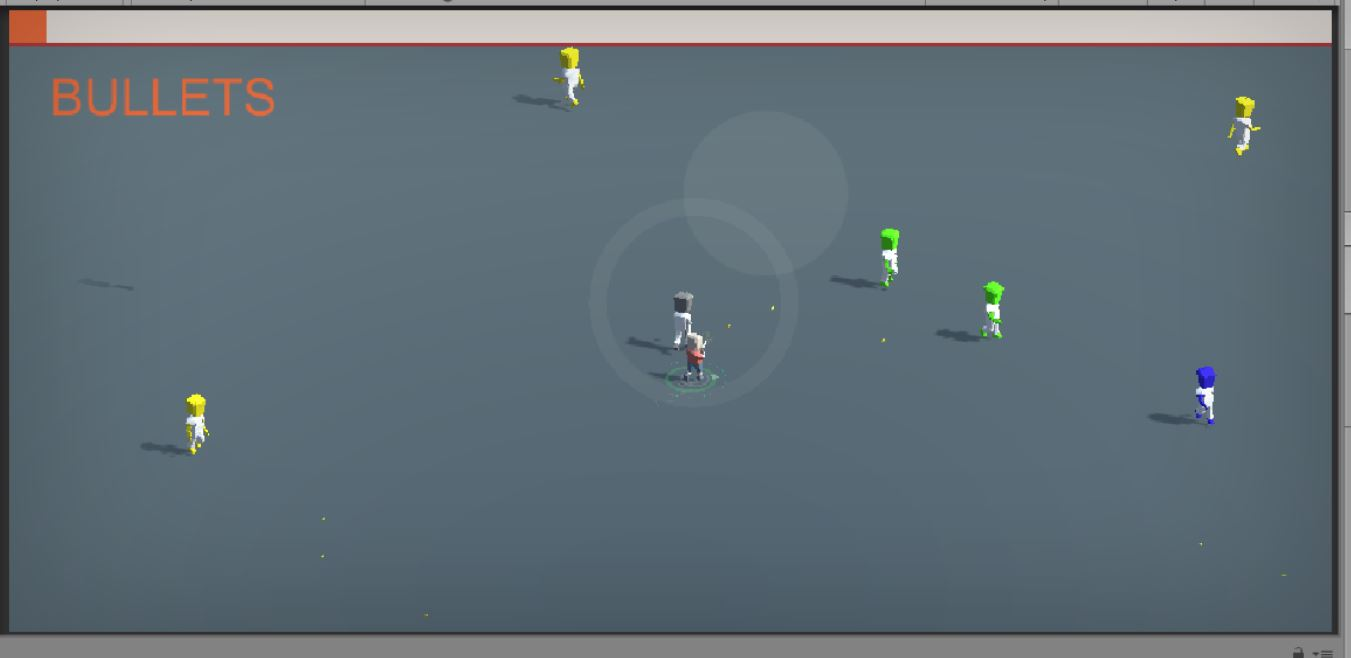
\includegraphics{Figures/bichi2.JPG}
\decoRule
\caption[Visualisation d'agents en état de joie]{Visualisation d'agents en état de joie}
\label{fig:bichi2}
\end{figure}


\subsection{Troisième expérimentation}

On ajoute cette fois-ci à l'expérience précédente un autre facteur émotionnel, celui de la tristesse, ce dernier intervient lorsque la distance équivaut à la valeur médiane entre les deux distances précédentes, c’est-à-dire un delta de 14f. [Figure \ref{fig:333f}]


\begin{figure}[th]
\centering
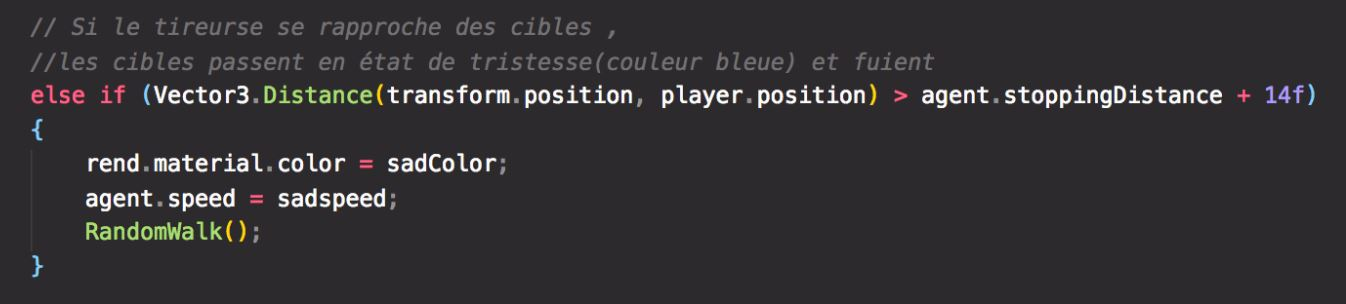
\includegraphics{Figures/333f.JPG}
\decoRule
\caption[Code source implémentant une distance médiane]{Code source implémentant une distance médiane entre le jouer et l'agent}
\label{fig:333f}
\end{figure}

~\par
Le résultat souhaité est de pouvoir appliquer un changement de couleur aux agents à l’instant où cette valeur médiane est atteinte. 


~\par
La couleur de ces derniers devient alors bleue, et leur vitesse passe à un rythme un peu plus soutenu que celui généré par la joie. [Figure \ref{fig:bichi3}]

\begin{figure}[th]
\centering
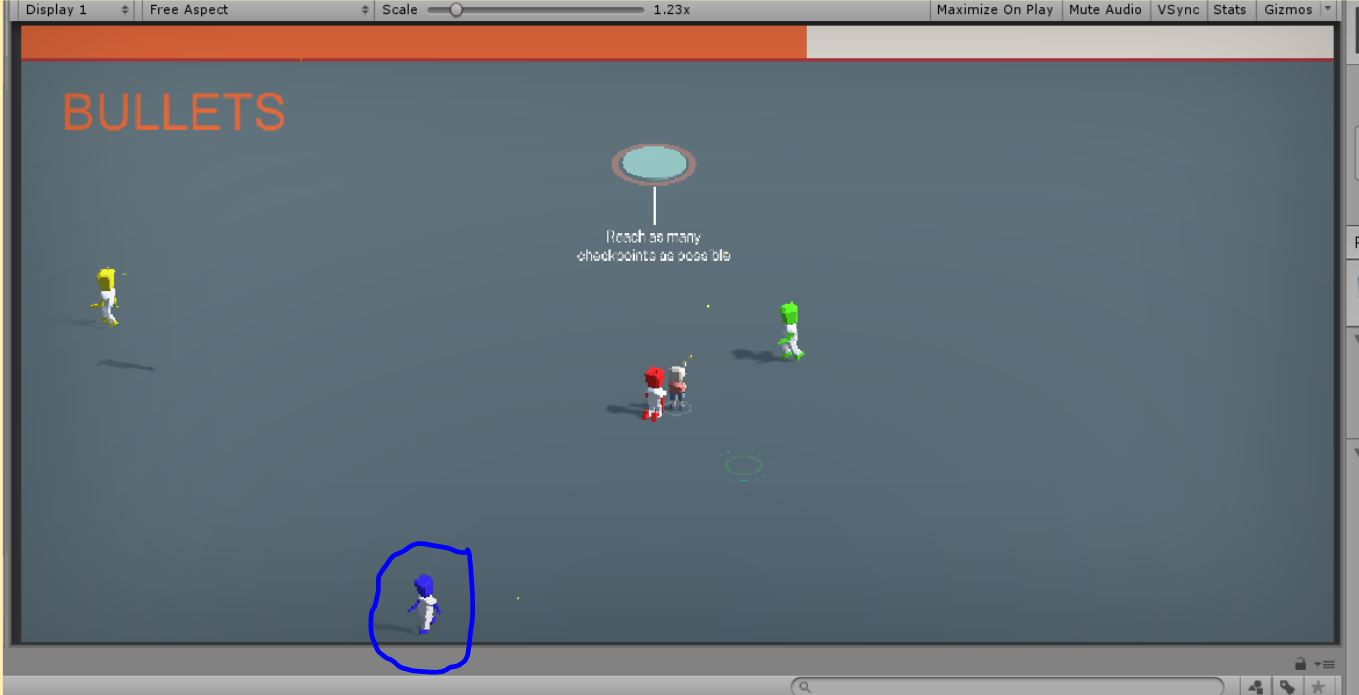
\includegraphics{Figures/bleu.JPG}
\decoRule
\caption[Visualisation d'agents en état de tristesse]{Visualisation d'agents en état de tristesse}
\label{fig:bichi3}
\end{figure}


~\par
Ajoutons à tout cela, le comportement présent dans le code source du jeu [Figure \ref{fig:derfon}], à savoir la colère, celle-ci génère une vitesse plus élevée que toutes les autres chez l’agent autonome, et une couleur noire(définie par moi), en plus de cela, elle change le centre d'intérêt du joueur en terme de démarche, jusque-là ce dernier se déplaçait de manière hasardeuse grâce à la fonction RandomWalk(), une fois le sentiment de colère déclenché, son point d’arrivée se rattache à la position du joueur(comme le montre la figure \ref{fig:bichi4} sur la page \pageref{fig:bichi4}).



\begin{figure}[th]
\centering
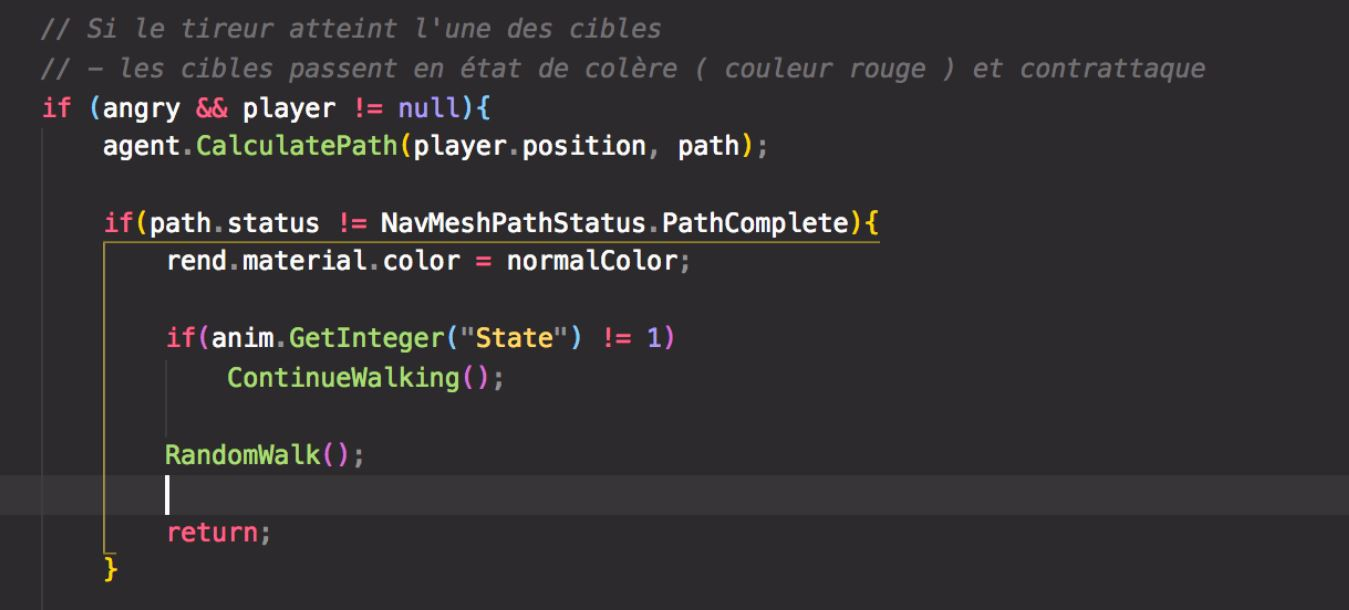
\includegraphics{Figures/derfon.JPG}
\decoRule
\caption[Code source implémentant la réaction d'un agent en état de colère]{Code source implémentant la réaction d'un agent en état de colère}
\label{fig:derfon}
\end{figure}



\begin{figure}[th]
\centering
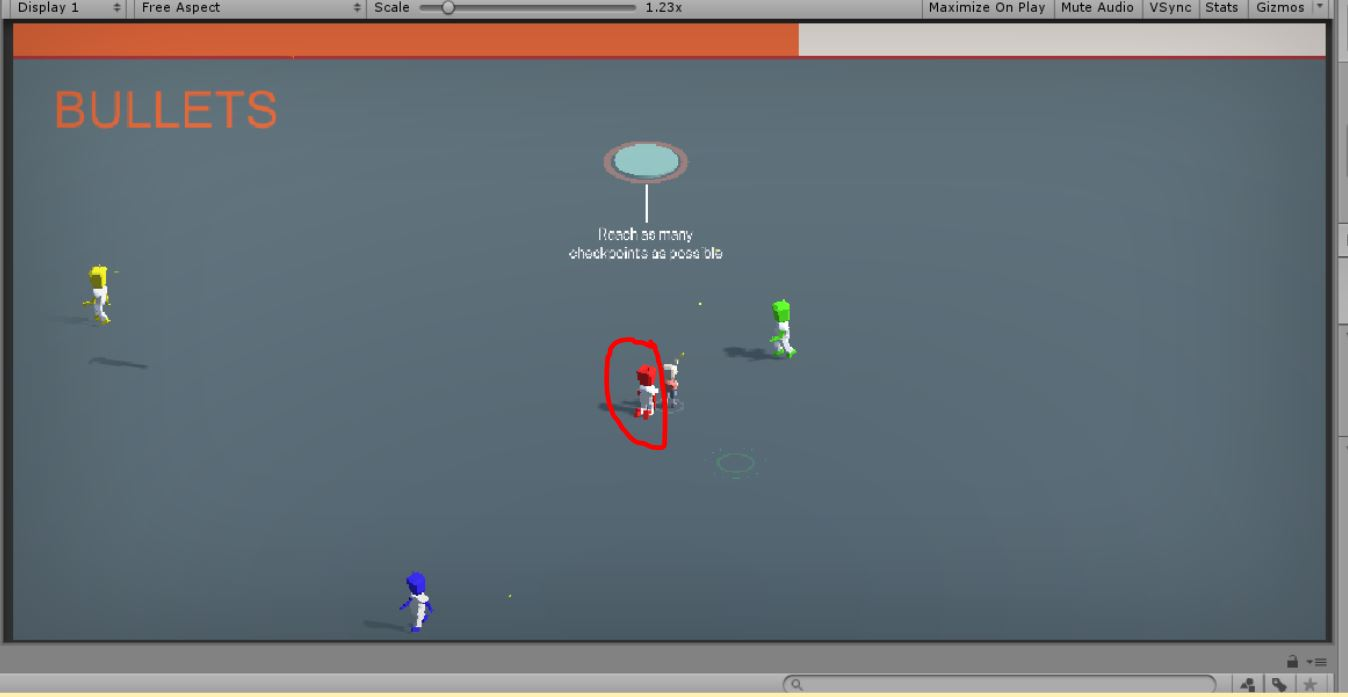
\includegraphics{Figures/rouge.JPG}
\decoRule
\caption[Visualisation d'agents en état de colère]{Visualisation d'agents en état de colère}
\label{fig:bichi4}
\end{figure}

\section{Résultat général (positif/négatifs)}

\subsection{Résultats positifs}

Les résultats suites à ces tests sont plutôt concluants, et confirment l’hypothèse mise en place par le modèle BDI.


~\par
À chaque changement de l’état du monde, rapprochement ou éloignement de l’agent représentant la menace, les paramètres considérées, de joie, de peur, de tristesse ou de colère changent et influent sur la réaction des agents et leur comportement.


~\par
Le passage entre différentes émotions fonctionne quant à lui aussi très bien, par exemple, si le joueur se rapproche beaucoup des agents, ceux-ci prennent peur et changent leurs démarches afin d’aller plus vite et de fuir, mais si l’agent s’éloigne d’eux, les agents reprennent petit à petit une démarche normale (jusqu’à ce que la distance les séparant soit assez élevé pour qu’ils puissent considérer qu’il n’y a plus de danger), ainsi qu’une couleur correspondant à leur nouvelle émotion.


~\par
On peut remarque les prises de décisions sont donc peu “rationnels”, et plus “naturels”, même si quelques points négatifs restent observables.

\subsection{Résultats négatifs}

L’un des points négatifs peut se résumer dans le passage d’une émotion à une autre qui n’est pas à mon sens pas assez réaliste, en effet dans la réalité, un agent humain peut mettre plusieurs minutes, plusieurs heures voient plusieurs jours ou mois pour se passer d’une émotion à une autre, ou se débarrasser d’une émotion désagréable liée à des situations particulières telles que des traumatismes.

~\par
Pouvoir appliquer cela dans un jeu vidéo, implique d'après moi d’ajouter des facteurs temporels à chaque émotion, facteur temporel d'acquisition de l’émotion et facteur temporel de disparition(dismiss) de l’émotion, ainsi que des facteurs d’intensité, en effet, les études sur les êtres humains montrent que toutes les émotions ne se valent pas en terme d’intensité, de manifestation physique ou psychologique.







